\documentclass[a4paper]{article}
\usepackage{svn-multi}
% Version control information:
\svnidlong
{$HeadURL: https://practicas-spss.googlecode.com/svn/trunk/intervalos_confianza/intervalos_confianza.tex $}
{$LastChangedDate: 2010-09-27 16:37:11 +0200 (lun, 27 sep 2010) $}
{$LastChangedRevision: 3 $}
{$LastChangedBy: asalber $}
\svnid{$Id: intervalos_confianza.tex 3 2010-09-27 14:37:11Z asalber $}
\pdfinfo{/CreationDate (D:\svnpdfdate)}
\svnRegisterAuthor{alf}{Alfredo Sánchez Alberca}

\usepackage[spanish]{babel}
\usepackage[utf8x]{inputenc}
\usepackage{amsmath}
\usepackage{macros}
\usepackage[dvips]{graphicx}
\usepackage{enumitem}
\usepackage{subfigure}
\usepackage[small,bf]{caption2}
\usepackage[top=3cm, bottom=3cm, left=2.54cm, right=2.54cm]{geometry}
\usepackage{fancyhdr}
\pagestyle{fancy}

\lhead{\textsc{Universidad San Pablo CEU}} \rhead{\textsl{\textsf{Departamento de Métodos Cuantitativos}}}
\renewcommand{\headrulewidth}{0pt}
\renewcommand{\floatpagefraction}{.8}
\renewcommand{\textfraction}{.1}
\setcaptionwidth{\textwidth} \addtolength{\captionwidth}{-40pt}
\captionstyle{indent} \setlength\captionindent{\parindent}

\makeatletter
\let\savees@listquot\es@listquot
\def\es@listquot{\protect\savees@listquot}
\makeatletter

\begin{document}
\sloppy
\practica{Práctica de Estadística con Statgraphics}{Intervalos de Confianza}
\bigskip

\section*{Fundamentos teóricos}

\subsection*{Inferencia Estadística y Estimación de Parámetros}
El objetivo de un estudio estadístico es doble: describir la
muestra elegida de una población en la que se quiere estudiar
alguna característica, y realizar inferencias, es decir, sacar
conclusiones y hacer predicciones, sobre la población de la
que se ha extraído dicha muestra.

La metodología que conduce a obtener conclusiones sobre la
población, basadas en la información contenida en la
muestra, constituye la \emph{Inferencia Estadística}.

Puesto que la muestra contiene menos información que la
población, las predicciones serán aproximadas. Por eso,
uno de los objetivos de la inferencia estadística es
determinar la probabilidad de que una conclusión sacada a
partir del análisis de una muestra, sea cierta, y por ello, se
apoya en la teoría de la probabilidad.

Cuando se desea conocer el valor de alguno de los parámetros
de la población, el procedimiento a utilizar es la
\emph{Estimación de Parámetros, }que a su vez se divide en
\emph{Estimación Puntual}, cuando damos un único valor
como estimación del parámetro poblacional considerado, y
\emph{Estimación por Intervalos}, cuando interesa conocer no
sólo un valor aproximado del parámetro sino también la
precisión de la estimación. En este último caso el
resultado es un intervalo, dentro del cual estará, con una
cierta confianza, el verdadero valor del parámetro
poblacional. A este intervalo se le denomina \emph{intervalo de
confianza}. A diferencia de la estimación puntual en que se
utiliza un único estimador, en la estimación por intervalo
emplearemos dos estimadores, uno para cada extremo del intervalo.

\subsection*{Intervalos de Confianza}
Dados dos estadísticos muestrales $L_1$ y $L_2$, se dice que el intervalo $I=[L_1,L_2]$ es un \emph{Intervalo de Confianza} para un parámetro poblacional
$\theta$, con \emph{nivel de confianza} $1-\alpha$ (o \emph{nivel de
significación} $\alpha $), si la probabilidad de que los estadísticos que determinan los límites del intervalo tomen valores tales que $\theta$ esté comprendido entre ellos, es igual a $1-\alpha$, es decir,
\[
P\left( L_{1}<\theta <L_{2}\right) =1-\alpha.
\]

Los extremos del intervalo son variables aleatorias cuyos valores
dependen de la muestra considerada. Es decir, los extremos
inferior y superior del intervalo serían $L_{1}\left(
X_{1},...,X_{n}\right) $ y $L_{2}\left(
X_{1},...,X_{n}\right) $ respectivamente, aunque habitualmente escribiremos $%
L_{1}$ y $L_{2}$ para simplificar la notación. Designaremos mediante $%
l_{1}$ y $l_{2}$ los valores que toman dichas variables para una
muestra determinada $\left( x_{1},...,x_{n}\right) .$

Cuando en la definición se dice que la probabilidad de que el
parámetro $\theta $ esté en el intervalo $\left(
L_{1},L_{2}\right) $ es $1-\alpha $, quiere decir que en el
$100\cdot \left( 1-\alpha \right) \ \% $ de las posibles muestras,
el valor de $\theta $ estaría en los correspondientes
intervalos $\left( l_{1},l_{2}\right) .$

Una vez que se tiene una muestra, y a partir de ella se determina
el intervalo correspondiente $\left( l_{1},l_{2}\right) $, no
tendría sentido hablar de la probabilidad de que el
parámetro $\theta $ esté en el intervalo $\left(
l_{1},l_{2}\right) $, pues al ser $l_{1}$ y $l_{2}$ números,
el parámetro $\theta $, que también es un número,
aunque desconocido, estará o no estará en dicho intervalo,
y por ello hablamos de confianza en lugar de probabilidad.

Así, cuando hablemos de un intervalo de confianza para el parámetro $\theta $ con nivel de confianza $1-\alpha $, entenderemos que
antes de tomar una muestra, hay una probabilidad $1-\alpha $ de
que el intervalo que se construya a partir de ella, contenga el
valor del parámetro $\theta .$

Cuando se realiza la estimación de un parámetro mediante
un intervalo de confianza, el nivel de confianza se suele fijar a niveles altos (los más habituales son $0.9$, $0.95$ o $0.99$), para tener una alta confianza de que el parámetro está dentro del intervalo. Por otro lado, también interesa que la amplitud del intervalo sea pequeña para
delimitar con precisión el valor del parámetro
poblacional (esta amplitud se conoce como \emph{error} o \emph{imprecisión} del intervalo).
Pero a partir de una muestra, cuanto mayor sea el
nivel de confianza deseado, más imprecisión tendrá el
intervalo que se obtenga, y si se impone que el intervalo de
confianza sea más preciso, el nivel de confianza
correspondiente será más pequeño. Por consiguiente,
hay que llegar a una solución de compromiso entre el nivel de
confianza y la amplitud del intervalo. No obstante, si con la
muestra disponible no es posible obtener un intervalo
suficientemente preciso con un nivel de confianza aceptable, hay
que emplear una muestra de mayor tamaño. Al aumentar el tamaño muestral se consiguen
intervalos más precisos sin disminuir el nivel
de confianza, o niveles de confianza más altos manteniendo la
precisión del intervalo.


\subsubsection*{Intervalos de confianza para la media}

Apoyándose en conclusiones extraídas del Teorema Central
del Límite y de las distribuciones en el muestreo para la media
muestral, y teniendo en cuenta tres factores de clasificación: la
población de partida en la que obtenemos la muestra sigue o no una
distribución Normal, la varianza de dicha población es conocida o
desconocida, y si la muestra puede o no considerarse grande
($n\geq30$); obtenemos las siguientes expresiones correspondientes
a los diferentes intervalos de confianza.

\subsubsection*{Intervalo de confianza para la media de una
población normal con varianza conocida en muestras de
cualquier tamaño}

\[
\left( \overline{x}-z_{\alpha /2}\cdot \dfrac{\sigma }{\sqrt{n}},\ \overline{%
x}+z_{\alpha /2}\cdot \dfrac{\sigma }{\sqrt{n}}\right)
\]

En la figura \ref{g:intervalomedia} aparece un esquema explicativo de la construcción de este intervalo.

\begin{figure}[h!]
\begin{center}
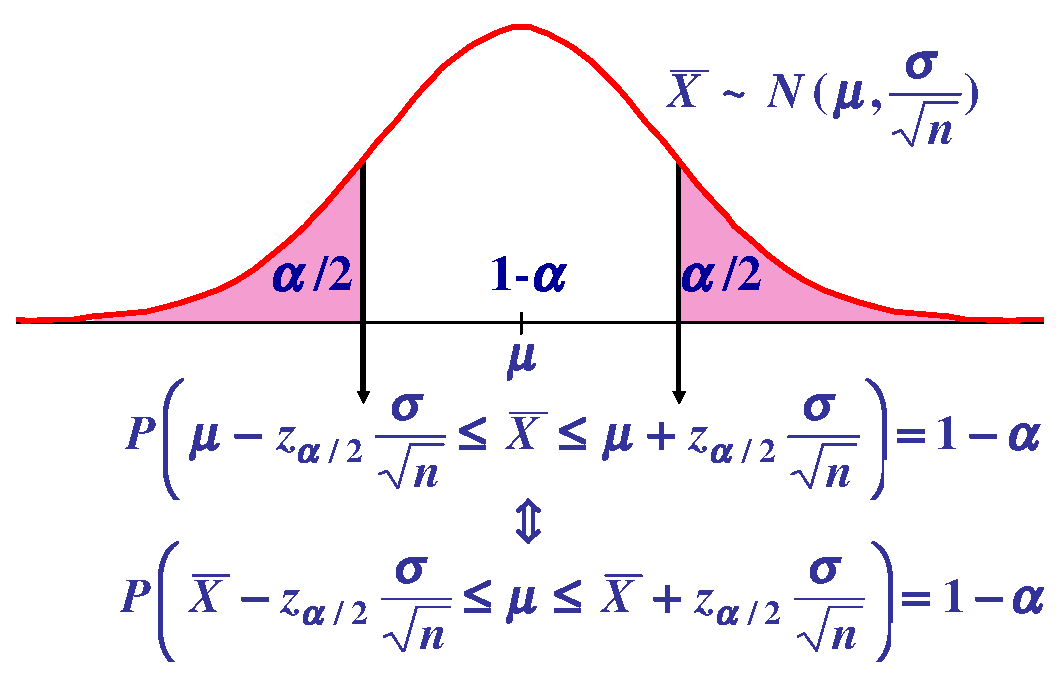
\includegraphics[scale=0.5]{intervalomedia.eps}
\caption{Intervalo de confianza para la media de una población
normal con varianza conocida.} \label{g:intervalomedia}
\end{center}
\end{figure}



\subsubsection*{Intervalo de confianza para la media de una población
normal con varianza desconocida en muestras de cualquier tamaño}

\[
\left( \overline{x}-t_{\alpha /2}^{n-1}\cdot
\dfrac{s_{n-1}}{\sqrt{n}},\ \overline{x}+t_{\alpha /2}^{n-1}\cdot
\dfrac{s_{n-1}}{\sqrt{n}}\right)
\]

Si las muestras son grandes ($n\geq30$) el anterior intervalo
puede aproximarse mediante:

\[
\left( \overline{x}-z_{\alpha /2}\cdot \dfrac{s_{n-1}}{\sqrt{n}},\ \overline{%
x}+z_{\alpha /2}\cdot \dfrac{s_{n-1}}{\sqrt{n}}\right)
\]



\subsubsection*{Intervalo de confianza para la media de una población no normal,
 varianza conocida y muestras grandes ($n\geq 30$)}

\[
\left( \overline{x}-z_{\alpha /2}\cdot \dfrac{\sigma }{\sqrt{n}},\ \overline{%
x}+z_{\alpha /2}\cdot \dfrac{\sigma }{\sqrt{n}}\right)
\]

\subsubsection*{Intervalo de confianza para la media de una población no normal,
 varianza desconocida y muestras grandes ($n\geq30$)}
\[
\left( \overline{x}-t_{\alpha /2}^{n-1}\cdot
\dfrac{s_{n-1}}{\sqrt{n}},\ \overline{x}+t_{\alpha /2}^{n-1}\cdot
\dfrac{s_{n-1}}{\sqrt{n}}\right)
\]

Al tratarse de muestras grandes, el anterior intervalo puede
aproximarse por:

\[
\left( \overline{x}-z_{\alpha /2}\cdot \dfrac{s_{n-1}}{\sqrt{n}},\ \overline{%
x}+z_{\alpha /2}\cdot \dfrac{s_{n-1}}{\sqrt{n}}\right)
\]

Si la población de partida no es normal, y las muestras son
pequeñas, no puede aplicarse el Teorema Central del Límite y no se
obtienen intervalos de confianza para la media.

Para cualquiera de los anteriores intervalos:

$n$ es el tamaño de la muestra.

$\overline{x}$ es la media muestral.

$\sigma $ es la desviación típica de la población.

$s_{n-1}$es la cuasidesviación típica muestral $\left( s_{n-1}^{2}=%
\dfrac{\sum \left( x_{i}-\overline{x}\right) ^{2}}{n-1}\right) $.

$z_{\alpha /2}$ es el valor que deja a su derecha una probabilidad
$\alpha /2 $ en una distribución normal tipificada.

$t_{\alpha /2}^{n-1}$ es el valor que deja a su derecha una probabilidad $%
\alpha /2$ en una distribución $t$ de Student con $n-1$ grados
de libertad.

\subsubsection {Intervalos de confianza para la diferencia de
medias}

De nuevo los criterios de clasificación de los diferentes
intervalos son el partir o no de poblaciones normales, con
varianza conocida o desconocida y en muestras grandes o pequeñas.

\subsubsection* {Intervalo de confianza para la diferencia de dos
medias en poblaciones normales, con varianzas poblacionales
conocidas, independientemente del tamaño de la muestra}

\[
\left( \overline{x}_{1}-\overline{x}_{2}-z_{\alpha /2}\cdot \sqrt{\dfrac{%
\sigma _{1}^{2}}{n_{1}}+\dfrac{\sigma _{2}^{2}}{n_{2}}},\ \overline{x}_{1}-%
\overline{x}_{2}+z_{\alpha /2}\cdot \sqrt{\dfrac{\sigma _{1}^{2}}{n_{1}}+%
\dfrac{\sigma _{2}^{2}}{n_{2}}}\right)
\]

\subsubsection* {Intervalo de confianza para la diferencia de dos
medias en poblaciones normales, con varianzas poblacionales
desconocidas, independientemente del tamaño de la muestra}


Si aún siendo desconocidas, las varianzas pueden considerarse
iguales, el intervalo es:

\[
\left( \overline{x}_{1}-\overline{x}_{2}-t_{\alpha
/2}^{n_{1}+n_{2}-2}\cdot
\sqrt{s_{p}^{2}\left( \dfrac{1}{n_{1}}+\dfrac{1}{n_{2}}\right) },\ \overline{%
x}_{1}-\overline{x}_{2}+t_{\alpha /2}^{n_{1}+n_{2}-2}\cdot \sqrt{%
s_{p}^{2}\left( \dfrac{1}{n_{1}}+\dfrac{1}{n_{2}}\right) }\right)
\]
donde $s_{p}^{2}$ es una cuasivarianza ponderada:

\[
s_{p}^{2}=\dfrac{\left( n_{1}-1\right) \cdot
s_{1,n_{1}-1}^{2}+\left( n_{2}-1\right) \cdot
s_{1,n_{2}-1}^{2}}{n_{1}+n_{2}-2}
\]

Si las varianzas, desconocidas, no pueden considerarse como
iguales, el intervalo es:

\[
\left( \overline{x}_{1}-\overline{x}_{2}-t_{\alpha /2}^{\nu }\cdot \sqrt{%
\dfrac{s_{1,n_{1}-1}^{2}}{n_{1}}+\dfrac{s_{2,n_{2}-1}^{2}}{n_{2}}},\
\overline{x}_{1}-\overline{x}_{2}+t_{\alpha /2}^{\nu }\cdot \sqrt{\dfrac{%
s_{1,n_{1}-1}^{2}}{n_{1}}+\dfrac{s_{2,n_{2}-1}^{2}}{n_{2}}}\right)
\]
donde $\nu$ es el número entero más proximo al valor de la
expresión:

\[
\dfrac{\left( \dfrac{s_{1,n_{1}-1}^{2}}{n_{1}}+\dfrac{s_{2,n_{2}-1}^{2}}{%
n_{2}}\right) ^{2}}{\dfrac{\left(
\dfrac{s_{1,n_{1}-1}^{2}}{n_{1}}\right)
^{2}}{n_{1}+1}+\dfrac{\left( \dfrac{s_{2,n_{2}-1}^{2}}{n_{2}}\right) ^{2}}{%
n_{2}+1}}-2
\]

Si los tamaños muestrales son grandes ($n_{1}\geq30$ y
$n_{2}\geq30$) las $t_{\alpha /2}^{\nu}$ y $t_{\alpha
/2}^{n_{1}+n_{2}-2}$ pueden sustituirse por $z_{\alpha/2}$.

\subsubsection* {Intervalo de confianza para la diferencia de dos
medias en poblaciones no normales, y muestras grandes
($n_{1}\geq30$ y $n_{2}\geq30$)}


En este caso, como ya sucedía con la media muestral, los
intervalos para la diferencia de medias son los mismos que sus
correspondientes en poblaciones normales y, de nuevo, habría que
distinguir si las varianzas son conocidas o desconocidas (iguales
o diferentes), lo cual se traduce en que sus correspondientes
fórmulas son las mismas que las dadas en los párrafos anteriores.
No obstante, por tratarse de muestras grandes, también es válida
la aproximación de $t_{\alpha /2}^{\nu}$ y $t_{\alpha
/2}^{n_{1}+n_{2}-2}$ por $z_{\alpha/2}$, y habitualmente tan sólo
se distingue entre varianzas conocidas y desconocidas.

Para varianzas conocidas:
\[
\left( \overline{x}_{1}-\overline{x}_{2}-z_{\alpha /2}\cdot \sqrt{\dfrac{%
\sigma _{1}^{2}}{n_{1}}+\dfrac{\sigma _{2}^{2}}{n_{2}}},\ \overline{x}_{1}-%
\overline{x}_{2}+z_{\alpha /2}\cdot \sqrt{\dfrac{\sigma _{1}^{2}}{n_{1}}+%
\dfrac{\sigma _{2}^{2}}{n_{2}}}\right)
\]
Para varianzas desconocidas:
\[
\left( \overline{x}_{1}-\overline{x}_{2}-z_{\alpha /2}\cdot \sqrt{%
\dfrac{s_{1,n_{1}-1}^{2}}{n_{1}}+\dfrac{s_{2,n_{2}-1}^{2}}{n_{2}}},\
\overline{x}_{1}-\overline{x}_{2}+z_{\alpha /2}\cdot \sqrt{\dfrac{%
s_{1,n_{1}-1}^{2}}{n_{1}}+\dfrac{s_{2,n_{2}-1}^{2}}{n_{2}}}\right)
\]

Si las poblaciones de partida no son normales y las muestras son
pequeñas, no puede aplicarse el Teorema Central de Límite y no se
obtienen intervalos de confianza para la diferencia de medias.

Para cualquiera de los anteriores intervalos:

$n_{1}$ y $n_{2}$ son los tamaños muestrales.

$\overline{x}_{1}$ y $\overline{x}_{2}$ son las medias muestrales.

$\sigma_{1} $ y $\sigma_{2} $ son las desviaciones típicas
poblacionales.

$s_{1,n_{1}-1}$ y $s_{2,n_{2}-1}$ son las cuasidesviaciones típicas muestrales: $s_{1,n_{1}-1}^{2}=%
\dfrac{\sum \left( x_{1,i}-\overline{x}_{1}\right) ^{2}}{n_{1}-1}
$, e igualmente $s_{2,n_{2}-1}^{2}$.

$z_{\alpha /2}$ es el valor que deja a su derecha una probabilidad
$\alpha /2 $ en una distribución normal tipificada.

$t_{\alpha /2}^{n_{1}+n_{2}-1}$ es el valor que deja a su derecha una probabilidad $%
\alpha /2$ en una distribución $t$ de Student con
$n_{1}+n_{2}-1$ grados de libertad.

$t_{\alpha /2}^{\nu}$ es el valor que deja a su derecha una probabilidad $%
\alpha /2$ en una distribución $t$ de Student con $\nu$ grados
de libertad.

\subsubsection {Intervalos de confianza para datos emparejados}
En muchas ocasiones hay que estudiar una característica en una
población en dos momentos distintos, para estudiar cómo
evoluciona con el tiempo, o para analizar la incidencia de
algún hecho ocurrido entre dichos momentos.

En estos casos se toma una muestra aleatoria de la población y
en cada individuo de la misma se observa la característica
objeto de estudio en los dos momentos citados. Así se tienen
dos conjuntos de datos que no son independientes, pues los datos
están emparejados para cada individuo. Por consiguiente, no se
pueden aplicar los procedimientos vistos anteriormente, ya que se
basan en la independencia de las muestras.

El problema se resuelve tomando para cada individuo la diferencia
entre ambas observaciones. Así, la construcción del
intervalo de confianza para la diferencia de medias, se reduce a
calcular el intervalo de confianza para la media de la variable diferencia, el
cual se obtiene aplicando las expresiones establecidas en 1.2.1.
Además, si cada conjunto de observaciones sigue una
distribución normal, su diferencia también seguirá una
distribución normal.

\subsubsection {Intervalos de confianza para proporciones y
diferencia de proporciones}

Para muestras grandes ($n\geq30~$) y valores de $p$ (probabilidad
de ``éxito'') cercanos a $0.5$, la distribución Binomial puede
aproximarse mediante una Normal de media $np$ y desviación típica
$\sqrt {np(1-p)}$. En la práctica, para que sea válida dicha
aproximación, se toma el criterio de que tanto $np$ como $n(1-p)$
deben ser mayores que 5. Y lo anterior hace que también podamos
construir intervalos de confianza para proporciones y diferencias
de proporciones tomando éstas como medias de variables dicotómicas
en las que la presencia o ausencia de la característica objeto de
estudio (``éxito'' ó ``fracaso'') se expresan mediante un 1 ó un 0.

\section*{Ejercicios prácticos}
\begin{enumerate}[leftmargin=*]
\item  Se analiza la concentración de principio activo en una
muestra de 10 envases tomados de un lote de un fármaco,
obteniendo los siguientes resultados en mg/mm$^{3}$:
\[
17.6 - 19.2 - 21.3 - 15.1 - 17.6 - 18.9 - 16.2 - 18.3 - 19.0 - 16.4
\]

Se pide:

\begin{enumerate}
\item  Crear la variable \variable{Concentración}, e introducir los
datos de la muestra.

\item  Calcular el intervalo de confianza para la media de la
concentración del lote con nivel de confianza del 95\% (nivel
de significación $\alpha =0.05$)
\begin{indicacion}{
\begin{enumerate}
\item Seleccionar el menú \menu{Descripción\flecha Datos Numéricos\flecha Análisis Unidimensional}.
\item Seleccionar la variable \variable{Concentración} en el campo \campo{Datos} del cuadro de diálogo.
\item Hacer click en el botón \boton{Opciones Tabulares} y activar la casilla \texttt{Intervalos de Confianza}.
\end{enumerate}}
\end{indicacion} 

\item Calcular los intervalos de confianza para la media con niveles del 90\% y
del 99\%.
\begin{indicacion}{
\begin{enumerate}
\item Hacer click con el botón derecho del ratón sobre los resultados obtenidos en el apartado anterior y seleccionar \texttt{Opciones de Ventana}.
\item Introducir el nivel de confianza deseado en el campo \campo{Nivel de Confianza}.
\end{enumerate}}
\end{indicacion} 

\item  ¿Cómo afecta a la imprecisión del intervalo de confianza el tomar niveles de significación cada vez más bajos? ¿Cuál puede ser la explicación?

\item  De todos los tipos de intervalos expuestos en la introducción teórica de la práctica, ¿cuál crees que utiliza el programa para el cálculo de los intervalos anteriores?

\item Si, para que sea efectivo, el fármaco debe tener una concentración
mínima de 16 mg/mm$^3$ de principio activo, ¿se puede aceptar el lote como bueno?
\end{enumerate}

\item  Para ver si una campaña de publicidad sobre un
fármaco ha influido en sus ventas, se tomó una muestra de
8 farmacias y se midió el número de unidades de dicho
fármaco vendidas durante un mes, antes y después de la
campaña, obteniéndose los siguientes resultados:
\[
\begin{tabular}{|c||c|c|c|c|c|c|c|c|}
\hline Antes & 147 & 163 & 121 & 205 & 132 & 190 & 176 & 147 \\
\hline Después & 150 & 171 & 132 & 208 & 141 & 184 & 182 & 145
\\ \hline
\end{tabular}
\]

\begin {enumerate}
\item Crear las variables \textsf{Antes} y \textsf{Después} e
introducir los datos de la muestra.

\item Obtener un resumen estadístico en el que aparezcan la media y la desviación típica de ambas variables. A la vista de los resultados, ¿son las medias diferentes?, ¿ha aumentado la campaña el nivel de ventas? ¿Crees que los resultados son estadísticamente significativos?
\begin{indicacion}{
\begin{enumerate}
\item Seleccionar el menú \menu{Comparación\flecha Dos Muestras\flecha Comparación de Dos Muestras}.
\item Seleccionar la variable \variable{Antes} en el campo \campo{Muestra 1} y la variable \variable{Después} en el campo \campo{Muestra 2} del cuadro de diálogo.
\item Hacer click en el botón \boton{Opciones Tabulares} y activar la casilla \texttt{Resumen Estadístico}.
\end{enumerate}}
\end{indicacion} 

\item Obtener intervalo de confianza para la media de la diferencia entre ambas variables con un nivel de significación $0.05$.
\begin{indicacion}{
\begin{enumerate}
\item Seleccionar el menú \menu{Comparación\flecha Dos Muestras\flecha Comparación Muestras Pareadas}.
\item Seleccionar la variable \variable{Antes} en el campo \campo{Muestra 1} y la variable \variable{Después} en el campo \campo{Muestra 2} del cuadro de diálogo.
\item Hacer click en el botón \boton{Opciones Tabulares} y activar la casilla \texttt{Intervalos de Confianza}.
\end{enumerate}}
\end{indicacion}

\item Crear la variable \variable{Diferencia} como \textsf{Después-Antes} y calcular el intervalo de confianza para la media de dicha variable con un nivel de significación del $0.05$. Comparar el intervalo obtenido con el del apartado anterior.
\begin{indicacion}{
\begin{enumerate}
\item Seleccionar el menú \menu{Descripción\flecha Datos Numéricos\flecha Análisis Unidimensional}.
\item Seleccionar la variable \variable{Diferencia} en el campo \campo{Datos} del cuadro de diálogo.
\item Hacer click en el botón \boton{Opciones Tabulares} y activar la casilla \texttt{Intervalos de Confianza}.
\end{enumerate}}
\end{indicacion} 

\item ¿Existen pruebas suficientes para afirmar con un 95\% de confianza que la campaña de publicidad ha aumentado las ventas? ¿Y si cambiamos los dos últimos datos de la variable \texttt{Después} y ponemos 190 en lugar de 182 y 165 en lugar de 145? Observar qué le ha sucedido al intervalo para la diferencia de medias y darle una explicación.
\end{enumerate}

\item  Una central de productos lácteos recibe diariamente la leche de dos granjas $X$ e $Y$. Para analizar la
calidad de la leche, durante una temporada, se controla el contenido de materia grasa de la leche que proviene de ambas granjas, con los siguientes resultados:
\[
\begin{array}{ll|ll}
\multicolumn{2}{c|}{X} & \multicolumn{2}{c}{Y} \\
\hline
0.34 & 0.34 & 0.28 & 0.29 \\
0.32 & 0.35 & 0.30 & 0.32 \\
0.33 & 0.33 & 0.32 & 0.31 \\
0.32 & 0.32 & 0.29 & 0.29 \\
0.33 & 0.30 & 0.31 & 0.32 \\
0.31 & 0.32 & 0.29 & 0.31 \\
 &  & 0.33 & 0.32 \\
 &  & 0.32 & 0.33 \\
\end{array}
\]

\begin{enumerate}

\item Crear las variables \textsf{Materia grasa} y \textsf{Granja}, e introducir los datos de la muestra.

\item Calcular el intervalo de confianza con un 95\% de confianza para la diferencia en el contenido medio de materia grasa de la leche procedente de ambas granjas.
\begin{indicacion}{
\begin{enumerate}
\item Seleccionar el menú \menu{Comparación\flecha Dos Muestras\flecha Comparación de Dos Muestras}.
\item Seleccionar la opción \opcion{Columnas de Códigos y Datos} e introducir la variable \variable{Materia Grasa} en el campo \campo{Datos} y la variable \variable{Granja} en el campo \campo{Código de Muestra} del cuadro de diálogo.
\item Hacer click en el botón \boton{Opciones Tabulares} y activar la casilla \texttt{Comparación de Medias}.
\end{enumerate}}
\end{indicacion}

\item Interpreta el intervalo de confianza obtenido en el apartado anterior.

\item De las fórmulas vistas en teoría, ¿cuál crees que utiliza el programa para el cálculo del intervalo del primer apartado, la que supone igualdad de varianzas en ambas muestras o la que no da por supuesta dicha igualdad?
\begin{indicacion}{
En la misma ventana de resultados del apartado anterior hacer click en el botón \boton{Opciones Tabulares} y activar la casilla \texttt{Comparación de Desviaciones Típicas}.}
\end{indicacion}

\end{enumerate}

\item En una encuesta realizada en una facultad, sobre si los
alumnos utilizan habitualmente (al menos una vez a la semana) la
biblioteca de la misma, se han obtenido los siguientes resultados,
en los que se ha anotado 1 si la respuesta ha sido positiva y 0 si
ha sido negativa:
\begin{center}
\begin{tabular}{l}
\begin{tabular}{|l|l|l|l|l|l|l|l|l|l|l|l|l|l|l|l|l|l|l|}
\hline
\multicolumn{1}{|c|}{Alumno} & \multicolumn{1}{c|}{1} & \multicolumn{1}{c|}{2} & \multicolumn{1}{c|}{3} & \multicolumn{1}{c|}{4} & \multicolumn{1}{c|}{5} & \multicolumn{1}{c|}{6} & \multicolumn{1}{c|}{7} & \multicolumn{1}{c|}{8} & \multicolumn{1}{c|}{9} & \multicolumn{1}{c|}{10} & \multicolumn{1}{c|}{11} & \multicolumn{1}{c|}{12} & \multicolumn{1}{c|}{13} & \multicolumn{1}{c|}{14} & \multicolumn{1}{c|}{15} & \multicolumn{1}{c|}{16} & \multicolumn{1}{c|}{17} & \multicolumn{1}{c|}{18} \\
\hline
\multicolumn{1}{|c|}{Sexo} & \multicolumn{1}{c|}{H} & \multicolumn{1}{c|}{M} & \multicolumn{1}{c|}{M} & \multicolumn{1}{c|}{H} & \multicolumn{1}{c|}{H} & \multicolumn{1}{c|}{H} & \multicolumn{1}{c|}{M} & \multicolumn{1}{c|}{M} & \multicolumn{1}{c|}{M} & \multicolumn{1}{c|}{M} & \multicolumn{1}{c|}{H} & \multicolumn{1}{c|}{H} & \multicolumn{1}{c|}{M} & \multicolumn{1}{c|}{H} & \multicolumn{1}{c|}{M} & \multicolumn{1}{c|}{H} & \multicolumn{1}{c|}{H} & \multicolumn{1}{c|}{M} \\
\hline
\multicolumn{1}{|c|}{Respuesta} & \multicolumn{1}{c|}{0} & \multicolumn{1}{c|}{1} & \multicolumn{1}{c|}{0} & \multicolumn{1}{c|}{0} & \multicolumn{1}{c|}{0} & \multicolumn{1}{c|}{1} & \multicolumn{1}{c|}{0} & \multicolumn{1}{c|}{1} & \multicolumn{1}{c|}{1} & \multicolumn{1}{c|}{1} & \multicolumn{1}{c|}{1} & \multicolumn{1}{c|}{0} & \multicolumn{1}{c|}{1} & \multicolumn{1}{c|}{0} & \multicolumn{1}{c|}{1} & \multicolumn{1}{c|}{0} & \multicolumn{1}{c|}{0} & \multicolumn{1}{c|}{0} \\
\hline
\end{tabular}\\
\\
\begin{tabular}{|l|l|l|l|l|l|l|l|l|l|l|l|l|l|l|l|l|}
\hline
\multicolumn{1}{|c|}{Alumno} & \multicolumn{1}{c|}{19} & \multicolumn{1}{c|}{20} & \multicolumn{1}{c|}{21} & \multicolumn{1}{c|}{22} & \multicolumn{1}{c|}{23} & \multicolumn{1}{c|}{24} & \multicolumn{1}{c|}{25} & \multicolumn{1}{c|}{26} & \multicolumn{1}{c|}{27} & \multicolumn{1}{c|}{28} & \multicolumn{1}{c|}{29} & \multicolumn{1}{c|}{30} & \multicolumn{1}{c|}{31} & \multicolumn{1}{c|}{32} & \multicolumn{1}{c|}{33} & \multicolumn{1}{c|}{34} \\
\hline
\multicolumn{1}{|c|}{Sexo} & \multicolumn{1}{c|}{H} & \multicolumn{1}{c|}{M} & \multicolumn{1}{c|}{M} & \multicolumn{1}{c|}{M} & \multicolumn{1}{c|}{H} & \multicolumn{1}{c|}{M} & \multicolumn{1}{c|}{H} & \multicolumn{1}{c|}{H} & \multicolumn{1}{c|}{M} & \multicolumn{1}{c|}{M} & \multicolumn{1}{c|}{H} & \multicolumn{1}{c|}{H} & \multicolumn{1}{c|}{M} & \multicolumn{1}{c|}{M} & \multicolumn{1}{c|}{M} & \multicolumn{1}{c|}{H}  \\
\hline
\multicolumn{1}{|c|}{Respuesta} & \multicolumn{1}{c|}{1} & \multicolumn{1}{c|}{1} & \multicolumn{1}{c|}{1} & \multicolumn{1}{c|}{0} & \multicolumn{1}{c|}{0} & \multicolumn{1}{c|}{1} & \multicolumn{1}{c|}{0} & \multicolumn{1}{c|}{0} & \multicolumn{1}{c|}{1} & \multicolumn{1}{c|}{1} & \multicolumn{1}{c|}{0} & \multicolumn{1}{c|}{0} & \multicolumn{1}{c|}{1} & \multicolumn{1}{c|}{0} & \multicolumn{1}{c|}{1} & \multicolumn{1}{c|}{0} \\
\hline
\end{tabular}
\end{tabular}
\end{center}

\begin{enumerate}
\item Crear las variables \textsf{Respuesta} y \textsf{Sexo} e introducir los datos de la muestra.

\item Calcular el intervalo de confianza con $\alpha=0.1$ para la media de la variable respuesta.
\begin{indicacion}{
\begin{enumerate}
\item Seleccionar el menú \menu{Descripción\flecha Datos Numéricos\flecha Análisis Unidimensional}.
\item Seleccionar la variable \variable{Respuesta} en el campo \campo{Datos} del cuadro de diálogo.
\item Hacer click en el botón \boton{Opciones Tabulares} y activar la casilla \texttt{Intervalos de Confianza}.
\item Hacer click con el botón derecho del ratón sobre los resultados obtenidos y seleccionar \texttt{Opciones de Ventana}.
\item Introducir el nivel de confianza deseado en el campo \campo{Nivel de Confianza}.
\end{enumerate}}
\end{indicacion}

\item ¿Qué interpretación tiene dicho intervalo en términos de proporción de alumnos que habitualmente utilizan la biblioteca?

\item Calcular el intervalo de confianza para la diferencia de proporciones de visitas a la biblioteca de hombres y mujeres. ¿Se puede afirmar con un 95\% de confianza que las mujeres visitan la biblioteca más a menudo que los hombres?
\begin{indicacion}{
\begin{enumerate}
\item Seleccionar el menú \menu{Comparación\flecha Dos Muestras\flecha Comparación de Dos Muestras}.
\item Seleccionar la opción \opcion{Columnas de Códigos y Datos} e introducir la variable \variable{Respuesta} en el campo \campo{Datos} y la variable \variable{Sexo} en el campo \campo{Código de Muestra} del cuadro de diálogo.
\item Hacer click en el botón \boton{Opciones Tabulares} y activar la casilla \texttt{Comparación de Medias}.
\end{enumerate}}
\end{indicacion}
\end{enumerate}


\end{enumerate}


\section*{Problemas}
\begin{enumerate}[leftmargin=*]
\item  Para determinar el nivel medio de colesterol en la sangre
de una población, se realizaron análisis sobre una muestra
de 8 personas, obteniéndose los siguientes resultados:
\[
196-212-188-206-203-210-201-198
\]

Hallar los intervalos de confianza para la media del nivel de
colesterol con niveles de significación $0.1$, $0.05$ y $0.01$.

\item  Se ha realizado un estudio para investigar el efecto del
ejercicio físico en el nivel de colesterol en la sangre. En el
estudio participaron once personas, a las que se les midió el
nivel de colesterol antes y después de desarrollar un programa
de ejercicios. Los resultados obtenidos fueron los siguientes:
\begin{center}
\begin{tabular}{|l|l|l|l|l|l|l|l|l|l|l|l|}
\hline
Nivel Previo & 182 & 232 & 191 & 200 & 148 & 249 & 276 & 213 & 241 & 280 & 262 \\
\hline
Nivel Posterior & 198 & 210 & 194 & 220 & 138 & 220 & 219 & 161 & 210 & 213 & 226 \\
\hline
\end{tabular}
\end{center}

\begin{enumerate}

\item Hallar el intervalo de confianza del 90\% para la
diferencia del nivel medio de colesterol antes y después del
ejercicio.

\item A la vista de dicho intervalo, ¿se concluye que el ejercicio
físico disminuye el nivel de colesterol con una confianza del 90\%?

\end {enumerate}

\item Dos químicos $A$ y $B$ realizan respectivamente 14 y 16 determinaciones de la actividad radiactiva de una muestra de material. Sus resultados en Curios:
\begin{center}
\begin{tabular}{ll|ll}
\multicolumn{2}{c|}{A} & \multicolumn{2}{c}{B} \\
\hline
263.36 & 254.68 & 286.53 & 254.54 \\
248.64 & 276.32 & 284.55 & 286.30 \\
243.64 & 256.42 & 272.52 & 282.90 \\
272.68 & 261.10 & 283.85 & 253.75 \\
287.33 & 268.41 & 252.01 & 245.26 \\
287.26 & 282.65 & 275.08 & 266.08 \\
250.97 & 284.27 & 267.53 & 252.05 \\
 &  & 253.82 & 269.81 \\
\end{tabular}
\end{center}
\begin{enumerate}
\item  Calcular el intervalo de confianza para la media de la
diferencia de actividad detectada por cada uno de los químicos con
un 95\% de confianza.

\item ¿Se puede decir que existen diferencias significativas en la
media de actividad detectada por cada químico?
\end{enumerate}

\end{enumerate}
\end{document}
